\chapter{Implementace}
\label{ch:implementation}
Tato sekce obsahuje popis implementace aplikace, která byla vytvořena na základě analýzy v předchozích kapitolách. V této sekci se tak zaměřím na popis jednotlivých komponent aplikace, které byly vytvořeny a následně nasazeny do produkce. Dále se zaměřím na popis týmové spolupráce, která byla nutná pro vytvoření celého projektu a na závěr se zaměřím na popis problémů, které se v průběhu vývoje objevily.

\section{Požadavky na implementaci}
\label{sec:implementation-requirements}

\section{Komponenty aplikace}
\label{sec:implementation-components}

\subsection{Frontend}
\label{subsec:implementation-frontend}

\subsection{Backend}
\label{subsec:implementation-backend}

\subsection{API}
\label{subsec:implementation-api}
Práce s API přes middleware, který zabezpečuje správné použití klíče.

\section{Volba technologií}
\label{sec:implementation-technologies}
V této sekci se budu věnovat výběru technologii které jsem zvolil v průběhu implmentace aplikace. Výběr technologii tak většinou vychází z analýzy uvedené v kapitole~\ref{ch:theory_and_analysis} nebo z osobních zkušeností, které jsem získal v průběhu studia.

\subsection{Framework}
\label{subsec:implementation-technologies-framework}
Jak bylo zmíněno v sekci analýze rozhraní, pro vývoj aplikace administrativního rozhraní jsem zvolil framework Django. Díky tomuto frameworku jsem tak mohl využít jeho širokou škálu již předem zakomponovaných funkcí, které mi usnadnily vývoj. Díky těmto funkcím jsem se mohl zaměřit na vývoj samotného rozhraní, které jsem tam psal v jazyce TypeScript s využitím frontendového frameworku Bootstrap.

Framework jako samotný neobsahuje rozšířené prvky pro použití na frontendu, z toho důvodu jsem byl nucen psát si tyto komponenty sám. Pro jejich vývoj jsem tam využil jazyk TypeScriptu, kde výsledné komponenty jsou mezi stránkami sdíleny. Pro dynamické načítaní obsahu je využíváno asynchronní načítání dat pomocí AJAXu, po prvotním načtení stránky zavoláno a po jeho zpracování dojde k překreslení části stránky.

Jedna z komponent, která slouží pro asynchronní získávaní dat je zobrazena v ukázce kódu~\ref{lst:data-request-component}. Tato komponenta slouží pro nahrazení dočasného obsahu na stránce obsahem který je získan v pozdějším procesu. Data jsou získány pomocí XMLHttpRequestu, který je volán na interní API, kde následně dochází k vyplnění obsahu templatu daty získanými z API a následně k jeho zobrazení.

\lstinputlisting[language=TypeScript, caption={Komponenta pro získání asynchronních dat.}, label={lst:data-request-component}]{sourceCodes/DataRequestComponent.ts}

\subsection{Knihovny}
\label{subsec:implementation-technologies-libraries}
Při vývoji aplikace jsem tak využil několik knihoven třetích stran, které mi tak usnadnily vývoj a zároveň zrychlily proces vývoje protože nebylo nutné psát vše od základu. Mezi tyto knihovny tak patří:

\begin{itemize}
    \item Font Awesome\footnote{\href{https://fontawesome.com/}{https://fontawesome.com/}} -- je knihovna ikon, která disponuje širokou škálou veřejně dostupných ikon, které jsou zdarma k použití. Ve vývoji jsem tak tyto ikony použil pro reprezentaci různých akcí, které může uživatel provést.
    \item Bootstrap\footnote{\href{https://getbootstrap.com/}{https://getbootstrap.com/}} -- jsem použil jako frontendovou knihovnu předem napsaný stylů, díky kterým jsem tak mohl rychle vytvořit efektivní a responzivní rozhraní. Bootstrap tak nabízí širokou škálu komponent, které jsou podrobně popsány v dokumentaci.
    \item SweetAlert2\footnote{\href{https://sweetalert2.github.io/}{https://sweetalert2.github.io/}} -- je knihovna, která umožnuje jednoduche zobrazovat nofikace a upozornění uživateli. Tato knihovna tak byla využita například pro zobrazení upozornění při chybě nebo úspěšném provedení akce.
    \item GoJS\footnote{\href{https://gojs.net/latest/index.html}{https://gojs.net/latest/index.html}} -- obsahuje funkce pro jednoduché a efektivní vytváření grafů, které byly využity pro interaktivní zobrazení návaznosti lokací na sebe.
    \item Animate.css\footnote{\href{https://animate.style/}{https://animate.style/}}, Hover.css\footnote{\href{https://ianlunn.github.io/Hover/}{https://ianlunn.github.io/Hover/}} -- jsou knihovny, které obsahuje před připravené animační styly, které stačí pouze aplikovat pomocí CSS tříd nebo dynamicky pomocí JavaScriptu.
    \item Notiflix\footnote{\href{https://notiflix.github.io/}{https://notiflix.github.io/}} -- je další z knihoven pro zobrazování notifikace, v tomto projektu jsem ale pro notifikace zvolil knihovnu SweetAlert2. Z toho důvodu je tato knihovna využita pouze pro blokaci uživatelského vstupu během načítání nebo zpracování dat formou loading spinneru.
    \item NoUISlider\footnote{\href{https://refreshless.com/nouislider/}{https://refreshless.com/nouislider/}} -- jedná se o knihovnu, které do prvků HTML přidává možnost vytvořit posuvníky, které je následně možné využit pro výběr hodnoty z rozsahu. Jeho příklad použití je v formuláři s filtrací dat.
\end{itemize}

\subsection{Jazykový procesor}
\label{subsec:implementation-technologies-compiler}
Výběr jazyka pro uživatelské rozhraní je důležitým aspektem v případě aplikací určených pro širokou veřejnost. V rámci této práce byl jako primární jazyk rozhraní zvolen jazyk anglický, což je nejuniverzálnější jazyk na světě. Díky čemuž je aplikace přístupná širokému spektru uživatelů bez potřeby překladu. Nicméně pro některé uživatele může být angličtina obtížná, a z toho důvodu byl implementován jazykový procesor, který umožňuje integraci více jazyků do aplikace.

Pro podporu vícejazyčné funkčnosti byla v této práci využita knihovna i18next\footnote{\href{https://www.i18next.com/}{https://www.i18next.com/}}, která je jednou z nejrozšířenějších nástrojů pro lokalizaci. Tato knihovna automaticky zpracovává jazykové soubory a aplikuje odpovídající překlady v závislosti na nastavení uživatele. Tímto způsobem je pro vývojáře snadné nastavit výchozí jazyk a později přidat další překlady.

\lstinputlisting[language=JavaScript, caption={Ukázka využití knihovny i18next.}, label={lst:i18next-example}]{sourceCodes/LanguageLocalization.js}

Na ukázce kódu~\ref{lst:i18next-example} je zobrazeno využití knihovny v případě obyčejného použití v JavaScriptu. Knihovna tak ale sama o sobě nabízí možnou integraci do různých frameworků jako například použitý freamework Django v této práci.

\subsection{Databáze}
\label{subsec:implementation-technologies-database}
Pro ukládání dat v našem systému jsme zvolili databázi MariaDB\footnote{\href{https://mariadb.org/}{https://mariadb.org/}}, která nám byla doporučena vedoucím práce. Nejedná se o nejmodernější databázi, ale o jednu s vysokou stabilitou a širokou historii použití. Databázi jsme tak pro bezpečnější použití rozdělili na dvě \textit{tts\_api} a \textit{tts\_api\_dev}, kde první obsahuje základní data a druhá data testovací. Pro vytvoření databáze byly následně využity scripty, které budou dále popsány v sekci automatizace.

\subsubsection*{Schéma}
\label{subsubsec:implementation-technologies-database-scheme}
Schéma databáze bylo vytvořena placeným softwarem DbDiagram.io\footnote{\href{https://dbdiagram.io/home}{https://dbdiagram.io/home}}, který tak nabízí možnost živého návrhu schémata, na kterým se tak mohl podílet každý člen týmu zároveň, což usnadnilo aktivní vývoj. Zkrácené schéma o n:n relacích je zobrazeno na obrázku~\ref{fig:db_scheme}. Software DbDiagram tak nabízí možnost exportu schématu do různých formátů, které byly následně využity pro vytvoření databáze v MariaDB\@.

\begin{figure}[H]
    \centering
    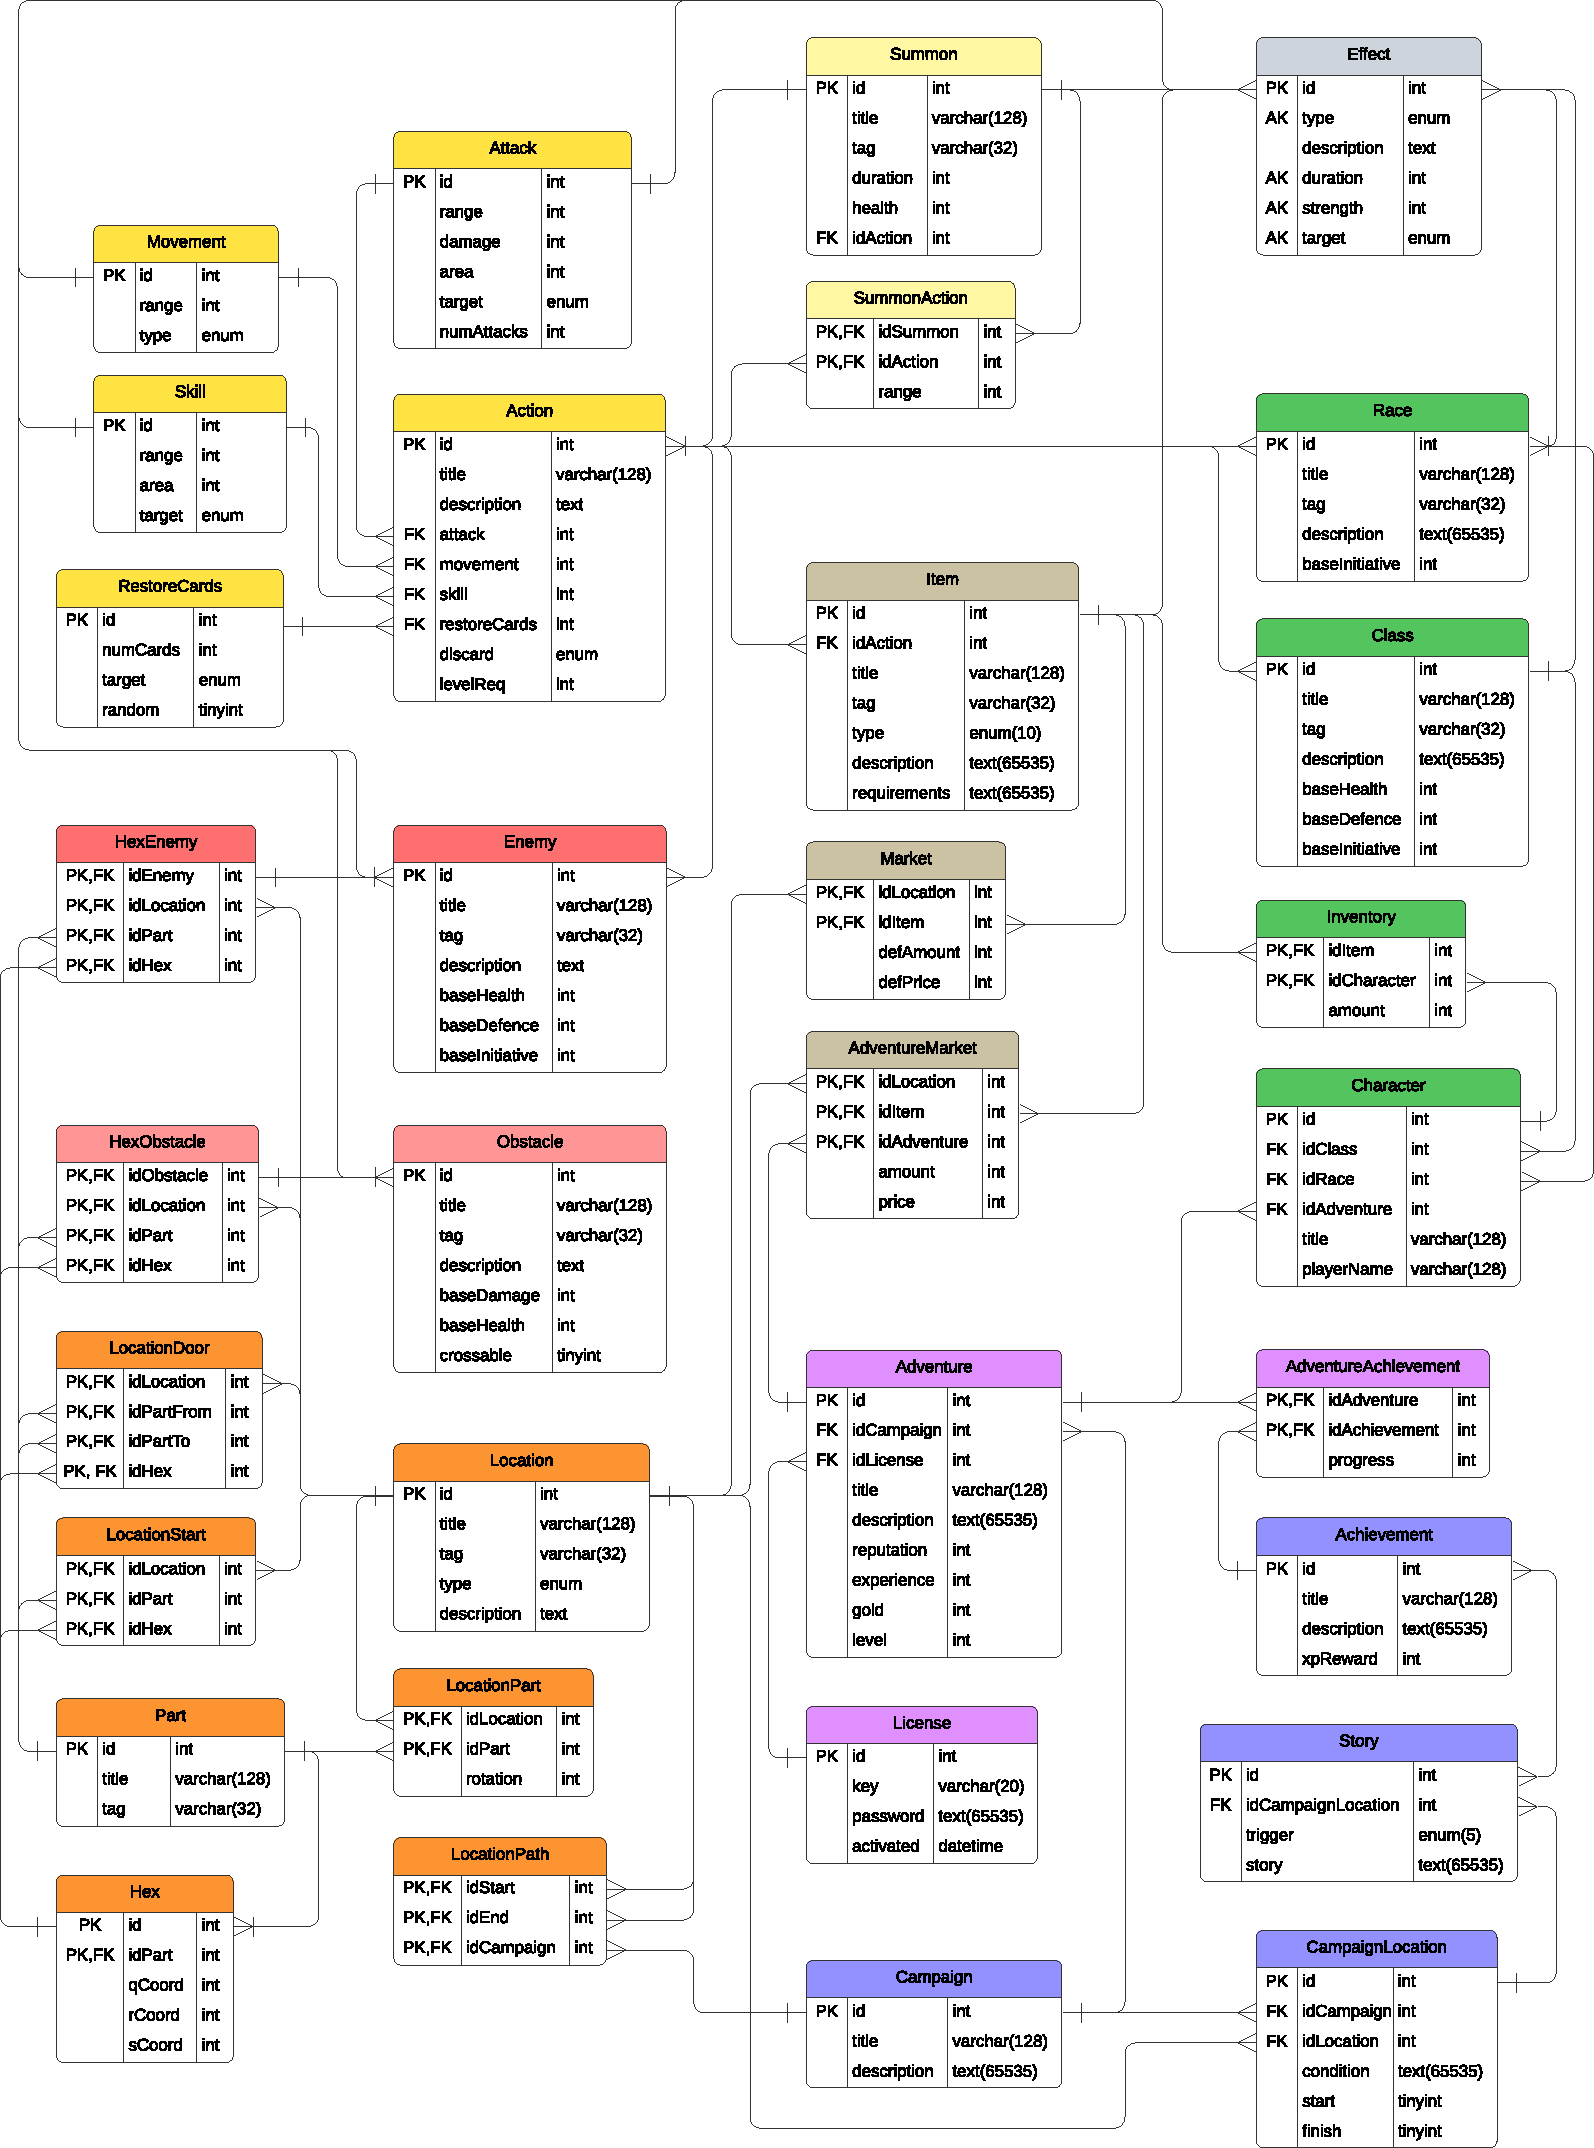
\includegraphics[width=0.96\textwidth]{../../shared/diagrams/dbScheme}
    \caption{Kompletní schéma databáze}
    \label{fig:db_scheme}
\end{figure}

\subsubsection*{Automatizace}
\label{subsubsec:implementation-technologies-database-automatization}
Automatizace vytváření a plnění databáze je důležitá pro kontinuální vývoj softwáru a v praxi se tak nazývá \textit{migrace}. Skripty pro vytvoření a naplnění databáze tak byly vytvořeny v skriptovacím jazyce Python\footnote{\href{https://www.python.org/}{https://www.python.org/}}. Tyto skripty tak byly vytvořeny tak, aby při jejich spuštění provedly kompletní smazání databáze, následně pak její znovu vytvoření a pozdější naplnění. Ukázka výstupu vytvořených scriptu je zobrazena v příloze~\ref{fig:databaseScriptsOutput}.

Pro vytvoření databáze byl použitý SQL soubory, který se po každé úpravě v nástroji DbDiagram.io zmíněným výše vyexportoval. Jakmile byla databáze resetována do výchozí podoby a vše proběhlo úspěšně. Došlo na řadu její plnění. Pro plnění databáze jsou data uloženy v souborech ve formátu JSON. Tyto soubory lze jednoduše exportovat z administračního rozhraní a uložit pro pozdější použití při obnově nebo plnění databáze.

Plnění databáze ale není jednoduchý proces, neboť je nutné zajistit správné pořadí cizích klíčů bez kterého se žádná tabulka nemůže bezchybně naplnit. Pro tento účet byl vytvořen diagram reprezentující abstraktní schéma databáze s prioritou jednotlivých tabulek, který je zobrazen na obrázku~\ref{fig:db_table_priority}. Tento diagram tak slouží jako návod pro správné nastavení priorit jednotlivých tabulek.

Pro čtení priority z grafu~\ref{fig:db_table_priority} je nutné vždy začít od dané tabulky a spočítat nejhlubší cestu k nejvzdálenější tabulce proti směru šipek. Tabulky s největší prioritou tak mají největší počet cest k sobě. V případě, že tabulka nemá žádnou cestu k sobě, je její priorita automaticky nastavena na 1. Tabulka priority je následně zobrazena v tabulce~\ref{tab:db_table_priority}.

\begin{figure}[H]
    \centering
    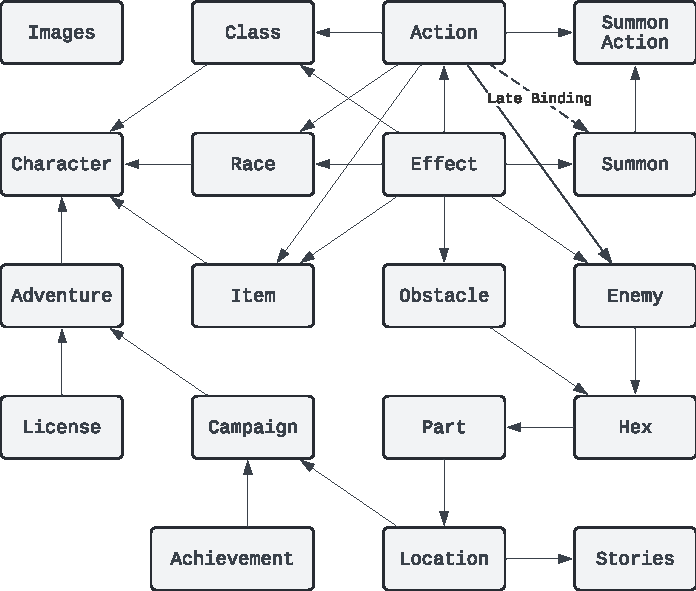
\includegraphics[width=0.7\textwidth]{diagrams/databasePriority}
    \caption{Schéma závislosti tabulek v databázi}
    \label{fig:db_table_priority}
\end{figure}

\begin{table}[H]
    \centering
        \begin{tabular}{l c l}
            \toprule

            \textbf{Název tabulky} & \textbf{Priorita} & \textbf{Závislost} \\
            \midrule

            \textbf{Effect} & 1 & -- \\
            \textbf{Achievement} & 1 & -- \\
            \textbf{Images} & 1 & -- \\
            \textbf{Parts} & 1 & -- \\
            \textbf{Obstacles} & 2 & Effect \\
            \textbf{Summons} & 2 & Effect \\
            \textbf{Enemies} & 3 & Effect, Action \\
            \textbf{Locations} & 3 & Part \\
            \textbf{Races} & 3 & Effect, Action \\
            \textbf{Items} & 3 & Effect, Action \\
            \textbf{Summons (Late Binding)} & 3 & Action \\
            \textbf{Campaigns} & 4 & Location, Achievement \\
            \textbf{Stories} & 4 & Location \\
            \textbf{Adventure} & 5 & License, Campaign \\
            \textbf{Characters} & 6 & Class, Race, Item, Adventure \\

            \bottomrule
        \end{tabular}
    \caption{Tabulka s prioritou dle diagramu~\ref{fig:db_table_priority}
    \label{tab:db_table_priority}}
\end{table}

\section{Týmová spolupráce}
\label{sec:implementation-collaboration}
Týmová spolupráce ve čtyřčlenném týmu studentů se stává obzvláště komplikovaná v době, kdy je projekt rozdělen do separátních části, které jsou na sebe závislé a je tak nutná vzájemná komunikace a spolupráce. Jako hlavní a nejvíce důležitou komponentou tohoto projektu se tak stává API, která slouží pro kompletní komunikaci v rámci projektu. V této sekci se tak zaměřím na to, jak jsme si rozdělili práci a jaký software jsme k tomu využili.

\subsection{Rozdělení práce}
\label{subsec:implementation-collaboration-distribution}
Rozdělení práce v týmu bylo provedeno tak, že každý člen měl dle zadání přidělenou určitou hlavní část projektu, za kterou byl plně zodpovědný. Každá z těchto částí projektu pak byla následně rozdělena na menší sekce, na kterých se daní členové podíleli buď samostatně nebo ve spolupráci. Spolupráce je tak zobrazena v šedém boxu, kde její vnitřní barevné čtverec reprezentuje daného člena. Ve výsledném rozdělení práce na obrázku~\ref{fig:job_distribution} je tak navíc jasně velikostně zobrazena náročnost jednotlivých částí projektu.

\begin{figure}[H]
    \centering
    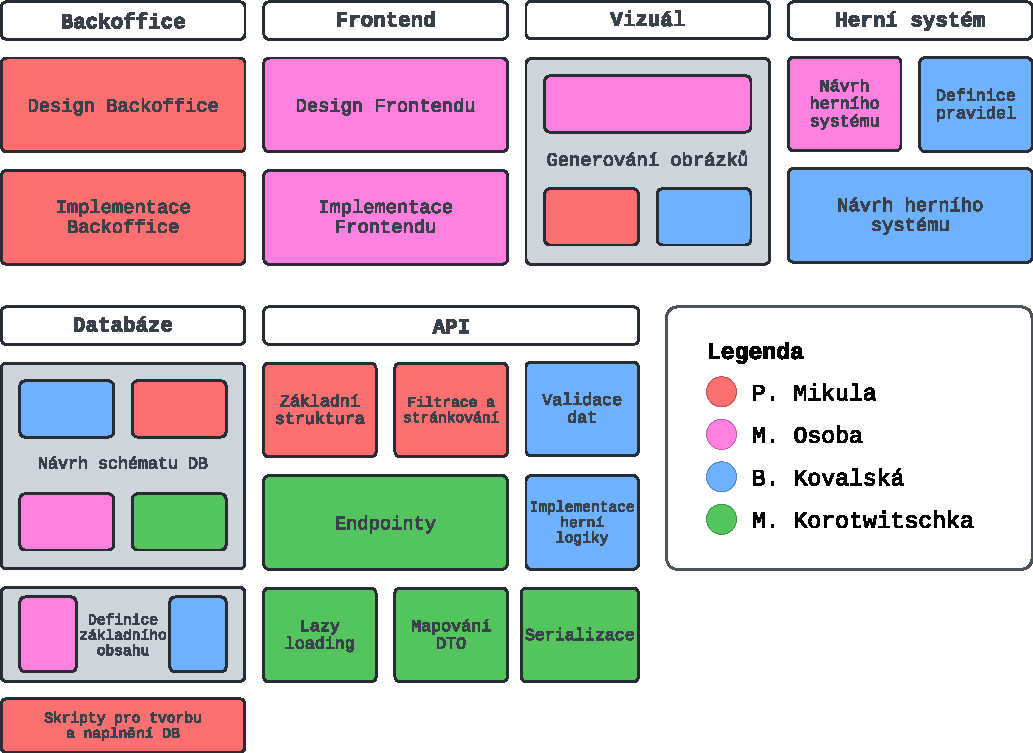
\includegraphics[width=0.95\textwidth]{../../shared/diagrams/blocks}
    \caption{Rozložení práce v týmu}
    \label{fig:job_distribution}
\end{figure}

\subsection{Verzování kódu}
\label{subsec:implementation-collaboration-versioning}
Efektivnost verzování kódu je důležitou součástí každé týmové spolupráce na větším projektu. Pro správu obsahu práce jsem tak využili nástroj Git pod službou GitHub\footnote{https://github.com/}, který nám umožnil efektivně sledovat změny a udržovat si tak přehled o vývoji projektu. Využití Gitu bylo zvoleno především pro jeho jednoduchost a znalost všech členů týmu, kteří s ním již měli zkušenosti v minulosti.

\subsubsection*{Větve}
\label{subsubsec:implementation-collaboration-versioning-branches}
V moderních vývojích systému se každá část nebo projekt celý rozděluje do složitějšího stromu větví známého pod názvem \textit{Git Worfkflow}, jeho efektivní reprezentace lze vidět na obrázku~\ref{fig:git_workflow}. Tento strom se dělí na vícero větví kde mezi ty hlavní tři větve patří \textit{live} neboli master, \textit{develop} a \textit{uat} známá jako testing branch.

Větev \textit{master} slouží pro produkční verze projektu, které jsou již plně připraveny k nasazení, zatímco větev \textit{develop} slouží pro vývoj nových funkcí případně oprav chyb. Při každém vývoji nové funkce se pak každá tato aktualizace dostává pomocí tzv. \textit{pull requestu} do větve testovací. V této větvi pak dochází k konstantnímu testování celého systému, pokuď je následně vše v pořádku. Aktualizace se dostávají do produkční větve.

Následně strom obsahuje pod větve vývojové, tyto větve se často štěpí z větve developu a slouží pro vývoj nových funkcí nebo opravu chyb. Po dokončení a úspěšném testování je tato větev spojena zpět do developu a po vydání nové verze je spojena do masteru.

\subsubsection*{Zkratky}
Tabulka zkratek zobrazena v obrázku ~\ref{fig:git_workflow}. Nejedná se zde o funkční příkazy softwaru Git, ale o pouhé zkratky pro přehlednější vyobrazení v schématu.

\begin{table}[H]
    \centering
    \resizebox{\textwidth}{!}{%
        \begin{tabular}{l l l}
            \toprule

            \textbf{Příkaz} & \textbf{Zkratka} & \textbf{Význam} \\
            \midrule

            \textbf{git nh} & New Hotfix & Vytvoření větve pro rychlou opravu chyb, která je již v produkci \\
            \textbf{git mh} & Merge Hotfix & Dokončení opravy chyby a spojení větve zpět do masteru \\
            \textbf{git live} & Release & Publikace nové verze a spojení větve do masteru \\
            \textbf{git nb} & New Bugfix & Vytvoření větve pro opravu chyb, která je ve vývoji \\
            \textbf{git mb} & Merge Bugfix & Dokončení vývoje a spojení větve zpět do developu \\
            \textbf{git uat} & User Acceptance Testing & Vytvoření větve pro testování nové verze \\
            \textbf{git nf} & New Feature & Vytvoření větve pro vývoj nové funkce \\
            \textbf{git mf} & Merge Feature & Dokončení vývoje a spojení větve zpět do developu \\

            \bottomrule
        \end{tabular}}
    \caption{Seznam zkratek pro větve v Git Workflow dle obrázku~\ref{fig:git_workflow}
    \label{tab:git_workflow}}
\end{table}

\begin{figure}[H]
    \centering
    \includegraphics[width=0.9\textwidth]{figures/GitWorkflow}
    \caption{Ukázka správného použití verzovacího systému Git. \cite{git_workflow}}
    \label{fig:git_workflow}
\end{figure}

\subsection{Sdílení kódu}
\label{subsec:implementation-collaboration-sharing}
Sdílení kódu není ve vývoji softwáru novinkou, neboť kód ve větším týmu spravuje vícero programátoru. Pro náš účel jsme tak opět použili systém \textit{GitHub}\footnote{https://github.com/}, kde po založení organizace dostávají všichni členové možnost zapojit se do vývoje. Obrázek~\ref{fig:git_organization} zobrazuje reprezentaci organizace na webové stránce \textit{GitHub}\footnote{https://github.com/Trails-Through-Shadows}, v nichž jsou zobrazeny jednotlivé části projektu, jejich krátky popis a jazyk, který v dané části převládá.

\subsection*{Rozdělení částí}
\label{subsec:implementation-collaboration-sharing-parts}
Při zakládaní organizace také došlo k zakoupení domény na kterou následně byly jednotlivé produkční verze nasazeny pomocí dalšího z nástrojů GitHubu a to \textit{GitHub Actions}\footnote{\href{https://github.com/features/actions}{https://github.com/features/actions}}, tento nástroj slouží pro automatizaci testování a následného nasazení funkční verze na server. Tento systém nám tak umožnil přehledný a automatický proces spuštění aplikace v praxi.

\noindent
V rámci organizace byly vytvořeny následující části:

\begin{itemize}
    \item TTS-Thesis    -- obsahuje texty diplomové práce od jednotlivých členů týmu se sdílenými materiály, který se taky nachází pod odkazem  \url{https://docs.tts-game.fun/thesis/intro}.
    \item TTS-Database  -- obsahuje skripty pro vytvoření a naplnění databáze základními daty, jejichž schéma je viditelné na obrázku~\ref{fig:db_scheme} nebo pod odkazem: \url{https://db.tts-game.fun}.
    \item TTS-API       -- obsahuje zdrojové kódy API, které slouží pro komunikaci mezi frontendem a backendem. Funkční produkční verze běží pod odkazem \url{https://api.tts-game.fun}.
    \item TTS-Dashboard -- obsahuje zdrojové kódy frontendu, který slouží pro zobrazení dat a správu aplikace. Produkční verze nalezena pod odkazem \url{https://dashboard.tts-game.fun}.
    \item TTS-Frontend  -- obsahuje frontend, který slouží pro interakci s uživatelem. Produkční verze dostupná na \url{https://play.tts-game.fun}.
    \item TTS-Docs      -- obsahuje dokumentaci k projektu která je volně dostupná pod odkazem \url{https://docs.tts-game.fun/data/intro}.
\end{itemize}

\begin{figure}[H]
    \centering
    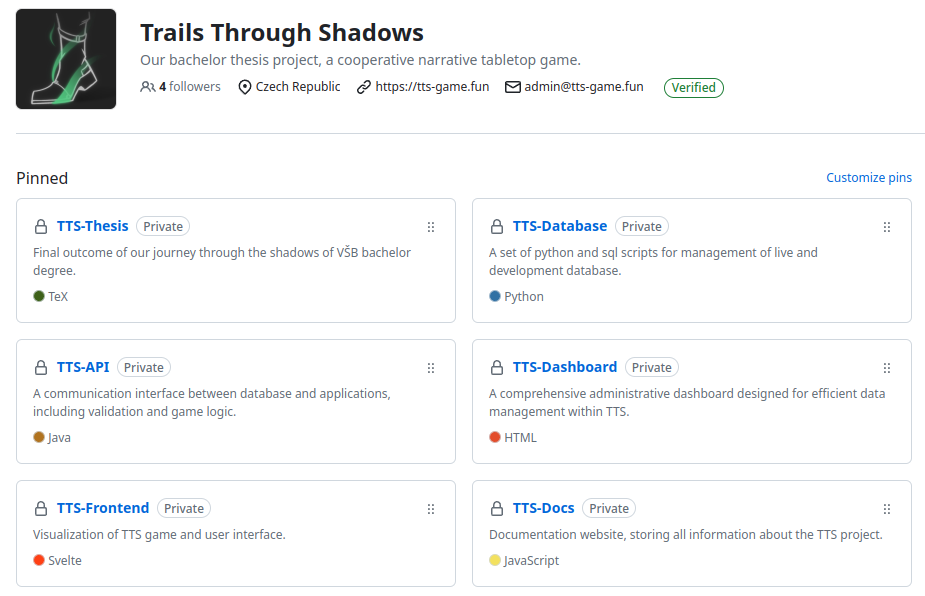
\includegraphics[width=0.9\textwidth]{../../shared/figures/gitOrg}
    \caption{Zobrazení organizace a jejich částí na stránce Github}
    \label{fig:git_organization}
\end{figure}

\subsection{Řešení problémů}
\label{subsec:implementation-collaboration-problems}
Pro řešení problému a chyb v softwaru, bylo pro tuto práci využito dalšího z nástrojů webu Github a to konkrétně \textit{Github Issues}\footnote{\href{https://github.com/features/issues}{https://github.com/features/issues}}, který slouží pro ukládání a monitoring problému v softwaru. Jako jednu z výhod tento nástroj přináší možnost přiřazení problému danému členovi nebo automatické vytvoření \textit{feature} větve a následného \textit{pull requestu}.

\section{Problémy vývoje}
\label{sec:implementation-problems}

\subsection*{Hexagonální grid}
\label{subsec:implementation-problems-hexagon}

\subsection*{Časová náročnost}
\label{subsec:implementation-problems-time}

\subsection*{Offset pro zobrazení partu}
\label{subsec:implementation-problems-offset}

\newpage
\processDiagram{diagrams/OpenPage}{OpenPage}{0.75\textwidth}{Diagram aaa}

\newpage
\processDiagram{diagrams/NewObject}{NewObject}{0.75\textwidth}{Diagram průběhu editace nebo přidávání dat}

\endinput